%\documentclass[notesonly, handout]{beamer}
\documentclass[]{beamer}

\usepackage[utf8]{inputenc}
\usepackage[T1]{fontenc}
\usepackage{listings}

% setup
\usetheme{Berlin}
\usecolortheme{beaver}
\setbeamercovered{transparent}
\hypersetup{pdfpagelabels=true}
\beamerdefaultoverlayspecification{<1->}
% \setbeamercovered{invisible}

% information
\title[Proto-Objects]{Proto-object based attention}
\subtitle{and the application to computer vision}
\author[Stephan Gabler] { \\\texttt{stephan.gabler@gmail.com}} 
\date[06/2011] {\today}

% set the logo
\pgfdeclareimage[height=1cm]{university-logo}{../images/bccn_logo.png}
\logo{\pgfuseimage{university-logo}}


\begin{document}

\section{Introduction} % (fold)
\label{sg:sec:introduction}



\frame{\titlepage}


\begin{frame}
    \note{why there is something like attention and what it possibly does}
    \note{in the end of the slide I say that there are also other theories of what attention does and where in the brain it is located, but all of them agree that attention does some selection}
    \note{broadbent  - 1958}
    \note{treisman - 1964}
    
    \frametitle{Attention}
    \framesubtitle{Why attention?}
    
    We cannot consciously attend to all sensory input at the same time.
    
    $\Rightarrow$ we have to select / prefer some stimuli over other
    \vspace{0.4cm}

    \begin{columns}
        \begin{column}{5cm}
            \onslide<2-3>{
                Broadbent's filter theory\\
                it is thought that attention serves as early selection.
            }
            \onslide<4>{...}
        \end{column}
        \begin{column}{5cm}
        \begin{overprint}
            \includegraphics<3>[width=4cm]{../images/selection.jpg}
        \end{overprint}
        \end{column}
    \end{columns}    
\end{frame}


\begin{frame}
    \note{if it is commonly accepted that there is some selection, how and what do we select?}
    \frametitle{Attention}
    \framesubtitle{Different kinds of attention / How do we chose?}
    
    bottom up $\rightarrow$ stimulus driven (physical stimulus properties)
    \begin{itemize}
        \item<1-> color
        \item<2-> luminance contrast
        \item<3-> motion
    \end{itemize}
    \uncover<4->{can be modeled/explained by saliency}
\includegraphics<4->[width=0.4\textwidth]{../images/saliency_example.png}
\end{frame}


\begin{frame}
    \note{mention that good results for saliency models came, because saliency is often correlated with object locations}
    \note{Fixations in an eye-tracker experiment (overt attention) can be explained better by object locations than by saliency.}
    \frametitle{Attention}
    \framesubtitle{Different kinds of attention / How do we chose?}

    top down $\rightarrow$ task-dependent (objects, categories)
    \begin{itemize}
        \item<1-> high-level: object features, scene structure
        \item<2-> mid-level: surface, occlusion, continuation 
    \end{itemize}
    
    \begin{columns}<3->
        \begin{column}{5cm}
            Recent results (Einhauser et. al. 2008) suggest that our attention is object-based. 
        \end{column}
        \begin{column}{5cm}
            \includegraphics<3->[width=0.9\textwidth]{../images/einhaus.jpg}
        \end{column}
    \end{columns}        
\end{frame}


\begin{frame}
    \note{So, if our attention is guided by objects, how is this possible. How can we attend to objects before we recognize them?}
    \frametitle{Attention}
    \framesubtitle{High-level attention -> Top-down problem}
    
    How can we attend to an object, before we recognize it?
    
    \vspace{1cm}
    $\Rightarrow$ proto-objects
    \vspace{0.2cm}
    
    potential objects might be computed by mid-level features.
\end{frame}


\begin{frame}
    \note{explain the idea of the project}
    \frametitle{Idea}
    \framesubtitle{Use high/mid-level attention in computer vision}
    
    How can his be used in computer vision?\\
    \vspace{0.5cm}
    Look for a very simple heuristics to spot potential objects.\\
    \vspace{0.5cm}
    $\Rightarrow$ The depth information of a 3D camera could be used to implement such a simple heuristics.
    
    
\end{frame}

% section introduction (end)


\section{Implementation} % (fold)
\label{sg:sec:implementation}

\begin{frame}
    \frametitle{Implementation}
    \framesubtitle{Data provided by kinect}
    \begin{columns}
        \begin{column}{5 cm} 
            \centering
            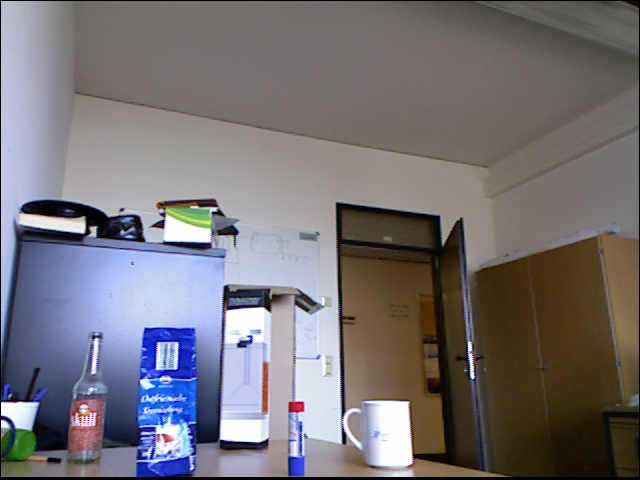
\includegraphics[width=5cm]{../images/image.jpg}
            
        \end{column}
        \begin{column}{5 cm}
            \centering
            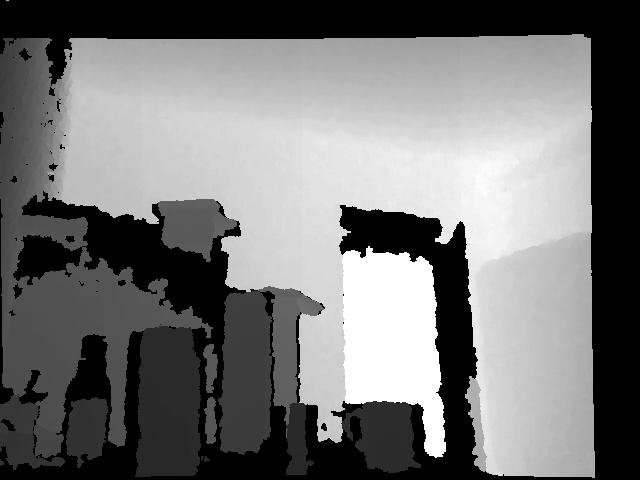
\includegraphics[width=5cm]{../images/depth.jpg}
        \end{column}
    \end{columns}
\end{frame}


\begin{frame}
    \frametitle{Algorithms and Results}
    \framesubtitle{histogram clustering (numpy)}
    \begin{figure}[h]
        \centering
            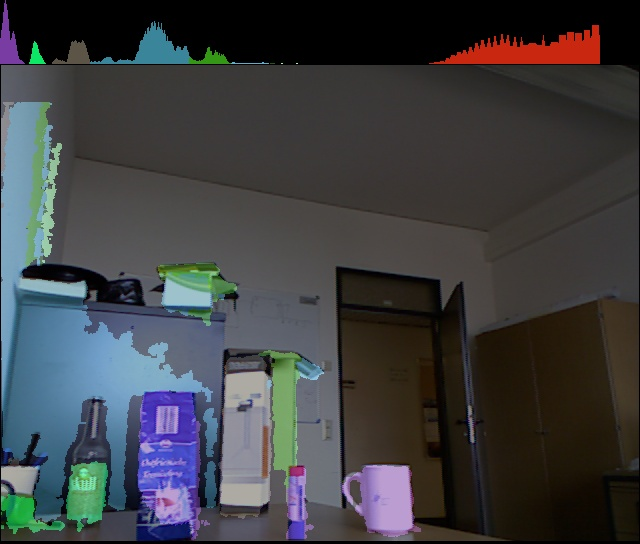
\includegraphics[height=0.6\textheight]{../images/cluster_bli_erode.jpg}
        \caption{Histogram clustering. patches colored by depth layer}
        \label{sg:fig:images_cluster_bli_erode}
    \end{figure}
\end{frame}


\begin{frame}
    \frametitle{Algorithms and Results}
    \framesubtitle{extract and filter contours (opencv)}
    \begin{figure}[h]
        \centering
    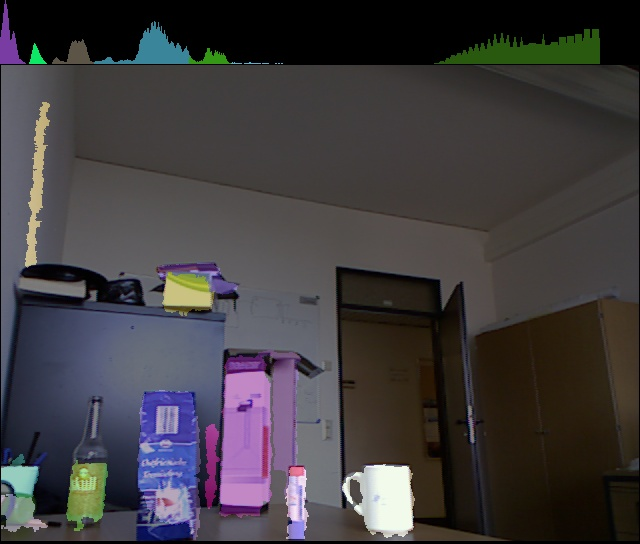
\includegraphics[height=0.6\textheight]{../images/extracted_contours.jpg}
        \caption{Extracted contours are filtered by simple heuristics (size, complexity)}
        \label{sg:fig:images_extracted_contours}
    \end{figure}
\end{frame}

\begin{frame}
    \frametitle{Algorithms and Results}
    \framesubtitle{morphological operator (opencv)}
    \begin{columns}
        \begin{column}{5 cm} 
        \begin{figure}[h]
            \centering
            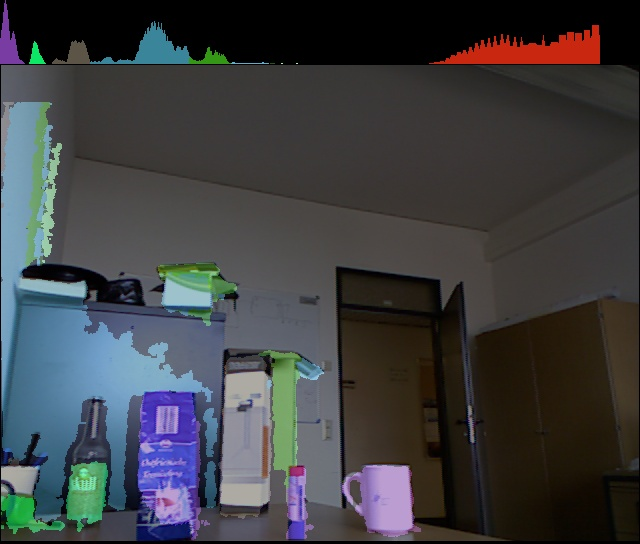
\includegraphics[width=5cm]{../images/cluster_bli_erode.jpg}
            \caption{before \emph{erosion}}
        \end{figure}
            
        \end{column}
        \begin{column}{5 cm}
            \begin{figure}[h]
                \centering
                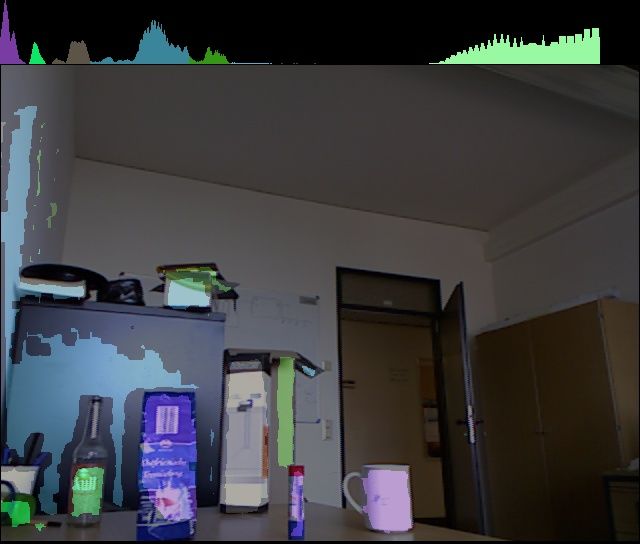
\includegraphics[width=5cm]{../images/cluster_im_erode.jpg}
                \caption{after \emph{erosion}}
            \end{figure}
        \end{column}
    \end{columns}
\end{frame}



\begin{frame}
    \frametitle{Algorithms and Results}
    \framesubtitle{Object tracking (opencv)}
    
    \begin{enumerate}
        \item<1-> keep a list of all previously detected objects
        \item<2-> extract the contours of all objects in current frame
        \item<3-> compute minimum bounding rectangle for the contours
        \item<4-> compute overlap of bounding rectangle with the one of the objects
        \item<5-> if overlap > 50\% of original size $\rightarrow$ object found
    \end{enumerate}
\end{frame}


% masking has the advantage that false positives are decreased
\begin{frame}
    \frametitle{Algorithms and Results}
    \framesubtitle{extract patch}
    
    Compute SIFT features if an object was constantly detected over N frames.
    
    \begin{itemize}
        \item<1-> extract patch in minimum bounding rectangle from the RGB image
        \item<2-> convert it to grayscale
        \item<3-> mask it by the contour
    \end{itemize}
    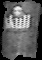
\includegraphics[width=1cm]{../images/image_sift_12.jpg}
    \hspace{0.1cm}
    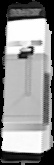
\includegraphics[width=1cm]{../images/image_sift_42.jpg}
    \hspace{0.1cm}
    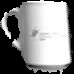
\includegraphics[width=1cm]{../images/image_sift_69.jpg}
    \hspace{0.1cm}
    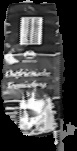
\includegraphics[width=1cm]{../images/image_sift_87.jpg}
    \hspace{0.1cm}
    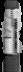
\includegraphics[width=1cm]{../images/image_sift_89.jpg}
\end{frame}

\begin{frame}
    \frametitle{Algorithms and Results}
    \framesubtitle{Object matching}
    
    The SIFT features found for each patch are then matched against a database of SIFT features using the FLANN library.
    \begin{figure}[h]
        \centering
            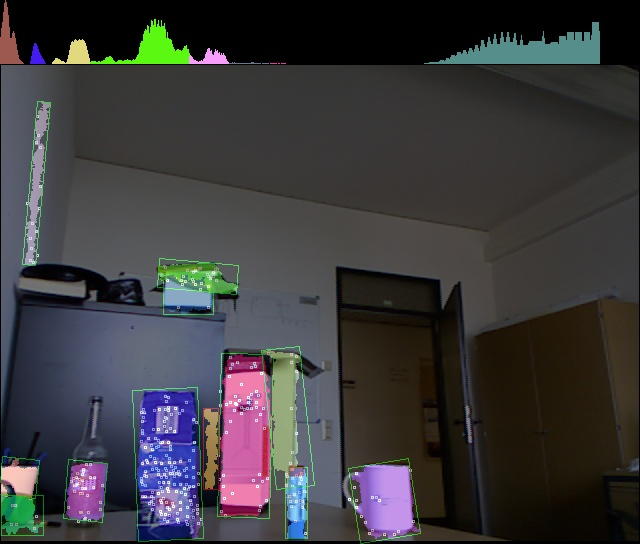
\includegraphics[height=0.6\textheight]{../images/contours_keypoints.jpg}
    \end{figure}
\end{frame}

% section implementation (end)

\section{Summary \& Outlook} % (fold)
\label{sg:sec:outlook}

\begin{frame}
    \frametitle{Summary}
    \framesubtitle{demonstration}
    
    videos ..
    
\end{frame}

\begin{frame}
    \frametitle{Summary}
    \framesubtitle{Results}
    
    \begin{itemize}
        \item<+-> faster SIFT computation because only on small patches
        % TODO add plot
        \item<+-> less false positives because patches masked by contour
    \end{itemize}
    
    \vspace{1cm}
    $\Rightarrow$ The concept of proto-objects can be used in computer-vision (even with a very simple heuristics)
    
\end{frame}


\begin{frame}
    \frametitle{Outlook}
    \framesubtitle{Further Ideas}
    \begin{itemize}
        \item<+-> use more advanced object tracking (e.g.: Kalman filter)
        \item<+-> maybe average over frames
        \item<+-> use color-histogram of objects for rough mapping
        \item<+-> iterative histogram clustering with neighboring condition
        \item<+-> multiprocess instead of multithread        
    \end{itemize}
\end{frame}

% section outlook (end)


\end{document}
